\documentclass[11pt,a4paper,sans]{moderncv} 

\moderncvstyle{classic} 
\moderncvcolor{blue} 
\usepackage{lipsum} 
\usepackage[utf8]{inputenc}
\usepackage[scale=0.85]{geometry} 
\usepackage{fontspec}
\newfontface\lserif{Liberation Serif}
\newcommand{\Csh}{C{\lserif\#}}
\firstname{El Hadiq} % Your first name
\familyname{Zouhair \href{https://orcid.org/0000-0002-6108-7176}{ 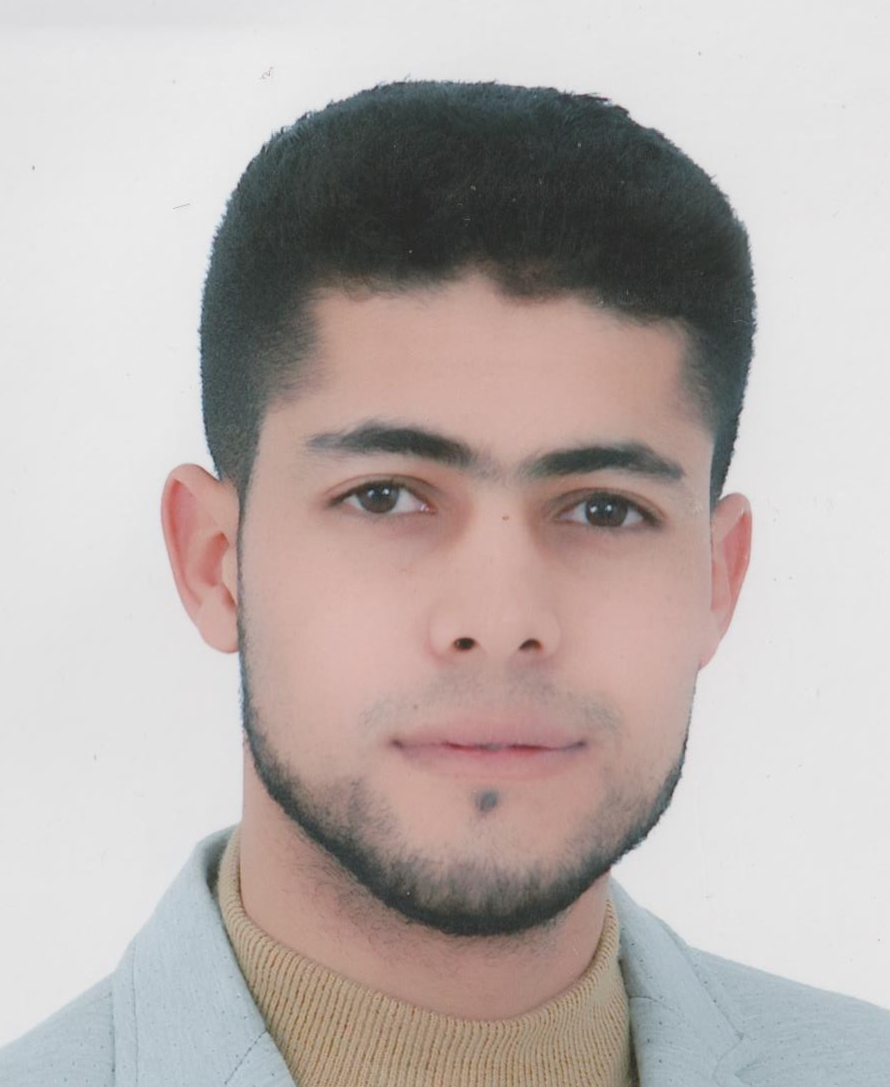
\includegraphics[scale=0.08]{mecv.jpg}}} % Your last name


\address{Quartier Al Qods N° 124 }{Guelmim, Morocco}
\mobile{(+212) 650 300 236}

\email{elhadiq.pro@gmail.com}
\quote{ \Large  Professeur Agrégé En Informatique\\ 
Ingénieur d’État en Modélisation et Informatique Scientifique}


\begin{document}

\makecvtitle 


%----------------------------------------------------------------------------------------
%	WORK EXPERIENCE SECTION
%----------------------------------------------------------------------------------------

\section{EXPERIENCES PROFESSIONNELLES}
\textbf{{Computer Science Professor}}\\
\cventry{2023--2025}{}{in preparatory classes MP \& PSI.}{}{}{CPGE Moulay Youssef, Rabat. }
\cventry{2022--2023}{}{in preparatory classes MP \& PSI.}{}{}{CPGE Moulay Youssef, Rabat. }
\cventry{2022--2023}{}{in preparatory classes MP \& PSI.}{}{}{CPGE Moulay Youssef, Rabat. }


\cventry{February--June 2019}{Final project}{Within the quantitative investment strategies team}{implementation of backtesting models for new quantitative investment strategies}{}{Société Générale Africa Technologies Services, Casablanca.}{}

\cventry{July--August 2018}{Engineering Internship}{Within the urban planning department}{realization of an adaptive controller for the traffic lights intersection}{}{NOVEC SA, Salé }

 \cventry{July--2017}{ Internship}{Within the computer and network department}{Development of a web application for absence management.}{}{OCP, Youssoufia.}


\section{Education}

\cventry{2020--2022}{Agrégation Informatique: Preparation for Agrégation in computer science.  }{}{}{}{CRMEF, Marrakech.} 
 
\cventry{2016--2019}{ Master's degree in Engineering: Modeling and Scientific Computing.  }{}{}{}{Ecole Mohammadia d’Ingénieurs, Rabat.}

\cventry{2015--2016}{Bachelor's degree In mathematics and computer sciences. 
 }{}{}{}{FST Guiliz, Marrakech}

\cventry{2013--2015}{Diploma of Higher University Studies in Science and Technology }{in Mathematics, physics and computer sciences}{}{}{FST Guiliz, Marrakech}

\cventry{2013}{High School Experimental Science Baccalaureate in Physics and Chemistry. }{}{}{}{Lycée  Kachkat, Youssoufia}


\section{Knowledge }

\cvitem{Fondamental }{Automata theory and proof theory,Logic,Complexity theory,compilation and analysis theory.}
\cvitem{Mathematics}{Probability,Calculus, Markov chaines, Optimisation, Quantitave finance, Market Finance}
\cvitem{Prgramming}{Java, C, Python, UML, SQL}
\cvitem{Systems and Tools}{GNU/Linux, Windows, System programming}

\section{Interests and Langages }
\cvitem{Langages}{English, French, and Arabe}
\cvitem{Interests}{ Camping, chess, harmonica, football, and theater. }
\end{document}